\subsection{openat}

\subsubsection{openat函数整体介绍}
openat函数用于打开文件。是 Linux 系统中用于打开文件的系统调用之一。它与 open 函数类似,但提供了更灵活和安全的文件路径处理方式。
openat() 在很多方面类似于 open(),但它提供了更加灵活和安全的文件路径处理方式:
\begin{itemize}
    \item 指定目录文件描述符: openat() 可以使用一个目录文件描述符作为起始位置,使得可以在指定目录下打开文件,而不受当前工作目录的影响。
    \item 相对路径打开: 可以使用相对于指定目录文件描述符的相对路径打开文件,避免了对当前工作目录的依赖。
\end{itemize}
openat的参数与返回值展示如下:
\begin{lstlisting}[language={Rust}, 
    caption={openat的参数与返回值}]
pub fn sys_openat(dirfd: usize, path: *const u8, flags: u32, mode: u32) -> isize
\end{lstlisting}
解释如下:
\begin{itemize}
    \item dirfd 是一个打开的目录文件描述符,用于指定相对路径的起始位置。可以是当前工作目录的文件描述符,或者是先前通过 open() 或 openat() 打开的目录文件描述符。
    \item path 是要打开的文件的路径名,可以是绝对路径或相对于 dirfd 的相对路径。
    \item flags 包含文件打开的标志,比如 O_RDONLY、O_WRONLY、O_CREAT、O_TRUNC 等,控制文件的打开方式。
    \item mode 是文件的权限设置,仅当 O_CREAT 被设置时才会生效,用于新建文件的权限设置。
\end{itemize}

\subsubsection{整体流程}
流程图展示如下:
\begin{figure}[H]
    \centering
    \scalebox{0.5}{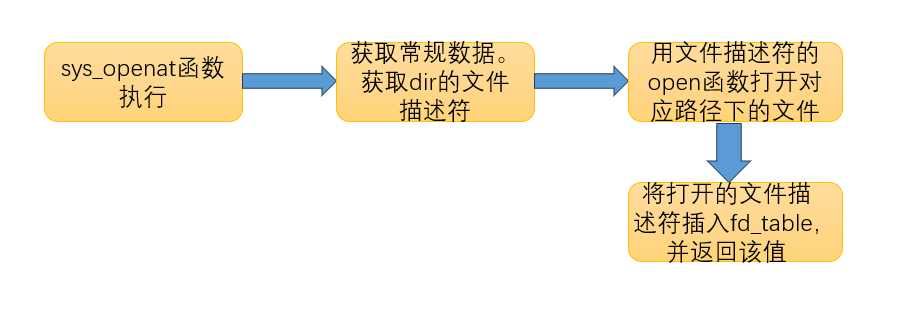
\includegraphics{figures/09-04-openat-函数流程.png}}
    \caption{execve流程图}
\end{figure}

\subsubsection{代码详析}
1、函数输入参数展示如下
\begin{lstlisting}[language={Rust}, 
    caption={openat的参数与返回值}]
pub fn sys_openat(dirfd: usize, path: *const u8, flags: u32, mode: u32) -> isize
\end{lstlisting}
2、常规操作,获取tcb信息,token,path、mode参数形式转换,获取fd_table
\begin{lstlisting}[language={Rust}, 
    caption={openat 常规操作,获取tcb信息、token、path参数形式转换}]
let task = current_task().unwrap();
let token = task.get_user_token();
let path = match translated_str(token, path) {
    Ok(path) => path,
    Err(errno) => return errno,
};
let flags = match OpenFlags::from_bits(flags) {
    Some(flags) => flags,
    None => {
        warn!("[sys_openat] unknown flags");
        return EINVAL;
    }
};
let mode = StatMode::from_bits(mode);
info!(
    "[sys_openat] dirfd: {}, path: {}, flags: {:?}, mode: {:?}",
    dirfd as isize, path, flags, mode
);
let mut fd_table = task.files.lock();
\end{lstlisting}
3、接着,函数尝试从当前任务的文件表(fd_table)中获取文件描述符。根据传入的 dirfd 参数,它会判断是否为特殊值 AT_FDCWD(表示当前工作目录),若不是则尝试从文件表中获取对应的文件描述符。
\begin{lstlisting}[language={Rust}, 
    caption={openat获取目录文件描述符}]
let file_descriptor = match dirfd {
    AT_FDCWD => task.fs.lock().working_inode.as_ref().clone(),
    fd => {
        let fd_table = task.files.lock();
        match fd_table.get_ref(fd) {
            Ok(file_descriptor) => file_descriptor.clone(),
            Err(errno) => return errno,
        }
    }
};
\end{lstlisting}
4、根据获取到的文件描述符,调用其 open 方法打开传入的 path 路径的文件,使用传入的 flags 和 mode。
如果打开成功,则将新的文件描述符加入到任务的文件表中,并返回该文件描述符作为结果。
\begin{lstlisting}[language={Rust}, 
    caption={openat-打开文件,返回值设置为文件描述符的}]
let new_file_descriptor = match file_descriptor.open(&path, flags, false) {
    Ok(file_descriptor) => file_descriptor,
    Err(errno) => return errno,
};

let new_fd = match fd_table.insert(new_file_descriptor) {
    Ok(fd) => fd,
    Err(errno) => return errno,
};
new_fd as isize
\end{lstlisting}
5、深入文件描述符的open函数。
总体来说,这段代码是文件描述符对象的 open 方法实现,用于处理文件系统中文件的打开操作。它检查路径是否有效,根据文件的类型进行不同的处理,最终尝试打开指定路径的文件或目录,并返回一个新的文件描述符对象或相应的错误信息。
首先,该方法接受三个参数:path(文件路径)、flags(打开文件的标志)、special_use(特殊用途标志)。
如果传入的路径 path 为空字符串 "",则直接返回当前文件描述符的克隆,即 Ok(self.clone())。
接着,如果当前文件描述符对应的文件是一个文件(不是目录),且传入的 path 不是以斜杠 / 开头(即相对路径),则返回错误 ENOTDIR(表示不是一个目录)。
之后,方法尝试从当前文件描述符对应的节点(即文件或目录)获取节点 inode。
如果成功获取到 inode,则调用 inode 的 open 方法,尝试以给定的 flags 和 special_use 打开传入的路径 path。如果打开成功,则获取到一个新的文件描述符 file。
根据传入的 flags 是否包含 O_CLOEXEC 标志,设置 cloexec 变量,用于指示是否在 file 上设置了 O_CLOEXEC(close-on-exec)标志。
最后,通过 Self::new() 创建一个新的文件描述符对象,返回一个包含新文件描述符的 Result。

\begin{lstlisting}[language={Rust}, 
    caption={文件描述符的open函数}]
    pub fn open(&self, path: &str, flags: OpenFlags, special_use: bool) -> Result<Self, isize> {
        if path == "" {
            return Ok(self.clone());
        }
        if self.file.is_file() && !path.starts_with('/') {
            return Err(ENOTDIR);
        }
        let inode = self.file.get_dirtree_node();
        let inode = match inode {
            Some(inode) => inode,
            None => return Err(ENOENT),
        };
        let file = match inode.open(path, flags, special_use) {
            Ok(file) => file,
            Err(errno) => return Err(errno),
        };
        let cloexec = flags.contains(OpenFlags::O_CLOEXEC);
        Ok(Self::new(cloexec, false, file))
    }
\end{lstlisting}

补充:O_CLOEXEC是在打开文件描述符时设置的一个标志,它表示在执行  execve()  调用时,该文件描述符将被关闭,避免子进程继承该文件描述符。

具体来说,当一个进程(父进程)打开一个文件描述符并设置了  O_CLOEXEC  标志后,如果在这个进程中调用  execve()  或  exec()  等系统调用来执行另一个程序,那么在新程序执行时,该文件描述符将会被自动关闭。这样可以确保新程序不会继承或意外使用父进程中打开的文件描述符,从而提高了安全性和可预测性。

这种行为通常用于父进程打开的文件描述符并不需要在子进程中保持打开的情况下。通过设置  O_CLOEXEC  标志,可以避免不必要的文件描述符传递到子进程中,减少了资源泄漏和意外的文件操作可能性。

6、文件目录树节点的open方法详析
这段 Rust 代码实现了 inode 对象的 open 方法,用于在文件系统中打开文件或目录。让我们逐步解析这段代码:

\textbf{日志记录和路径重定向:}

代码开始处记录了调试日志,包括当前工作目录和传入的路径。
接着定义了一些特殊路径和相应的重定向规则,例如将特定路径重定向到 BUSYBOX_PATH 或 LIBC_PATH 等。
经过一系列的条件判断,根据特定规则将传入的 path 重新赋值,以便后续处理。

\textbf{定打开的起始节点(inode):}

根据传入的 path 是否以 / 开头来确定打开文件的起始节点 inode,如果以 / 开头则从根节点(ROOT)开始,否则从当前节点(self)开始。

\textbf{路径缓存和文件系统操作:}

\begin{itemize}
    \item 使用互斥锁 PATH_CACHE.lock() 获取路径缓存,如果存在缓存且路径匹配,则直接使用缓存的 inode。\
    \item 否则,解析路径并逐级切换目录,获取到最终的目标 inode。
    \item 如果打开的文件不存在,根据标志位创建新的文件。
    \item 在文件存在的情况下,根据传入的标志位进行相应的操作,比如截断文件或检查文件状态。
\end{itemize}

\textbf{文件打开及特殊处理:}

\begin{itemize}
    \item 在文件打开之前,进行了一系列的检查,例如判断是否是目录、文件是否正在被使用、是否需要截断文件等。
    \item 根据 special_use 参数进行特殊处理,如果需要特殊处理,则增加 spe_usage 的计数值。
    \item 如果路径以 / 开头且与路径缓存不同,则更新路径缓存。
\end{itemize}

\textbf{返回结果:}

最后调用文件对象的 open 方法打开文件,根据操作结果返回成功打开的文件或相应的错误码。

7、深入OSInode的open方法

\textbf{创建文件对象:}

方法接受两个参数:flags(打开文件的标志)和 special_use(特殊用途标志)。
根据传入的标志位,设置文件对象的一些属性,比如 readable 表示文件是否可读、writable 表示文件是否可写、append 表示是否在末尾追加写入数据等。

\textbf{构建新的文件对象:}

使用 Arc::new() 创建一个新的文件对象 Arc<dyn File>。
在构建文件对象时,将文件对象的各种属性设置为对应的标志位状态或传入的参数状态,比如可读性、可写性、追加写入等。
将原始文件对象的内部状态 inner 进行克隆,offset 采用 Mutex 进行多线程安全的偏移量管理。

最后将创建的对象返回

\begin{lstlisting}[language={Rust}, 
    caption={OSInode的open方法}]
fn open(&self, flags: OpenFlags, special_use: bool) -> Arc<dyn File> {
    Arc::new(Self {
        readable: flags.contains(OpenFlags::O_RDONLY) || flags.contains(OpenFlags::O_RDWR),
        writable: flags.contains(OpenFlags::O_WRONLY) || flags.contains(OpenFlags::O_RDWR),
        special_use,
        append: flags.contains(OpenFlags::O_APPEND),
        inner: self.inner.clone(),
        offset: Mutex::new(0),
        dirnode_ptr: self.dirnode_ptr.clone(),
    })
}
\end{lstlisting}